%!TEX root = BCD.tex
 
%\section*{Introduction}

\par Molecular binding processes are ubiquitous in biology and serve as the 
fundamental basis for biological complexity. %Binding describes the event where 
%the preferential interactions of two molecules in proximity causes them to 
%associate. This is a key component for processes ranging from signaling cascades 
%and regulation to enzymatic catalysis. Binding also describes processes such as 
%protein-drug interactions, and engineered host-guest systems which span a broad 
%range of applications including catalysis, drug delivery, and 
%biotechnology\cite{DelValle2004,Davis2004,Ma2015a}.
For the drug discovery community, engineering pharmacologically active small molecules is of 
particular importance. Traditionally, the paradigm for lead optimization is to 
select for leads with the greatest affinity for a protein, or other, target of 
interest. However, recent evidence suggests that the kinetics of binding may 
also be a useful metric for lead selection. It is now thought that both residence 
times and association rates are key determinants of \textit{in vivo} efficacy 
for many drugs\cite{Schuetz2017,Lu2010a,Copeland2006b,Copeland2016,Swinney2004b}. 
Similar to computational predictions of binding thermodynamics, molecular 
simulations can be used to compute binding kinetics\cite{DeVivo2016,Amaro2018,Bruce2018a}. Methods such as Brownian 
Dynamics (BD) have been used effectively for estimating molecular
association rates\cite{Northrup1984,McCammon1986,Zhou1990,Huber2010}. 
%BD 
%approximates the rigid body diffusion of molecules interacting with the far-field
%electrostatics of a target. Owing to these simplifications BD calculations are 
%extremely fast but neglect molecular motion and detailed intermolecular 
%interactions.
%On the other hand, 
Molecular dynamics (MD) simulations 
which explicitly represent all atoms and forces, can also be used to predict 
binding kinetics. Due to significantly increased model complexity, MD is 
limited by sampling. Nevertheless, owing to software improvements and the 
development of commodity hardware such as GPUs and specialty hardware such as 
Anton\cite{Shaw2009,Shaw2014}, ``brute force'' calculation of binding kinetics with MD is now 
a possibility\cite{Shan2011,Shan2012,Dror2011,Pan2013a,Tang2017}. To improve 
upon ``brute force'' sampling statistics, many sampling strategies 
employ force biases or other statistical mechanical techniques to predict
both association and dissociation rates of many systems. This includes methods 
such as: Markov State Models\cite{Buch2011b,Plattner2015a,Wu2016,Doerr2014},
metadynamics\cite{Mollica2016a,Tiwary2015,Casasnovas2017}, 
milestoning\cite{Elber2017,Ma2017,Kirmizialtin2012,Yu2015,Bucci2016,Ma2015,Ma2017}, 
and other techniques\cite{Teo2016,Dickson2016,Dickson2017,Lotz2018a,Chiu2016,Wong2018,Tran2018}.

\par Our previous work uses a multiscale MD, BD, and Milestoning approach for 
the calculation of both association and dissociation rates of receptor-ligand 
complexes\cite{Votapka2015,Votapka2017}. Our implementation, %of this simulation scheme,
``Simulation Enabled Estimation 
of Kinetic Rates'' (SEEKR) 
is a freely available software package\footnote{https://amarolab.ucsd.edu/seekr} that automates the preparation, 
simulation, and analysis of these multiscale milestoning calculations using 
existing softwares: NAMD\cite{Phillips2005} for MD simulations and 
BrownDye\cite{Huber2010} for BD simulations. 
Milestoning theory
provides the glue for the multiscale scheme by providing a strategy to subdivide,
simulate, and subsequently statistically reconnect small regions of simulation 
space called ``milestones''\cite{Faradjian2004,Shalloway2006,West2007,Vanden-Eijnden2008,
Vanden-Eijnden2009,Majek2010,Kirmizialtin2011,Cardenas2013,Cardenas2015,
Bello-Rivas2015,Votapka2015,Votapka2017,Elber2017} This approach reduces the compute time required to simulate transition events, is embarrassingly parallel, and is agnostic to the simulation modality used. %The two key quantities
%necessary for the estimation of kinetics with milestoning are the transition kernel, 
%which contains the probability of transitioning from each milestone to all other 
%milestones, and an incubation time vector containing the average time spent in 
%each milestone. 
%By subdividing space into milestones, milestoning drastically
%reduces the compute time required to simulate transition events. 
%More importantlyfor our approach, 
%since both the transition kernel and incubation time are local
%to a specific milestone, 
%Furthermore, since each milestone is independent,
%the simulations are embarrassingly parallel but also
%agnostic to the simulation modality and physics used to obtain statistics.
%estimate these key 
%measurables.
This allows us to use atomically detailed, yet computationally expensive, 
fully flexible MD simulations in milestones near the binding site where these 
interactions are critical for understanding the binding and unbinding, and BD 
simulations far from the binding site where rigid body dynamics provides a 
sufficient description at significantly reduced computational cost. For a more 
thorough description of milestoning theory and the calculation of kinetic 
quantities, such as \kon and \koff, we refer the reader to the existing 
literature.\cite{Faradjian2004,Shalloway2006,West2007,Vanden-Eijnden2008,
Vanden-Eijnden2009,Majek2010,Kirmizialtin2011,Cardenas2013,Cardenas2015,
Bello-Rivas2015,Votapka2015,Votapka2017,Elber2017} 

%\par 
%Since each milestone is completely 
%independent, SEEKR runs each milestone in a parallel fashion and is limited only 
%by the availability of compute resources. Sampling enhancement results from 
%diffusive processes experiencing both a reduction in simulation time proportional to 
%the number of milestones and exponential bootstrapping/statistical ratcheting 
%which aids in the climbing of free energy barriers, resulting in a net savings that 
%is exponential with respect to number of milestones\cite{West2007}.

\par The effectiveness of the SEEKR scheme for the calculation of \kon and \koff 
values has been demonstrated for multiple protein-ligand systems\cite{Votapka2015,Votapka2017}.
However, it has not yet been used for rank ordering sets of compounds by kinetic 
(\kon and \koff) and thermodynamic ($\Delta G$) values, as would be done in
pharmaceutical discovery settings. Here we use SEEKR to estimate \kon , \koff, and $\Delta G$ 
for a model host-guest system, $\beta$-cyclodextrin with seven ligands 
representing diverse chemical groups (Fig.~\ref{fig:BCD_ligands}), using two  
forcefields for $\beta$-cyclodextrin  GAFF\cite{Wang2004,Wang2006} and Q4MD\cite{Cezard2011}. We compare the SEEKR estimates with previously
published ``brute force'' (long-timescale) MD predictions\cite{Tang2017} and experimental 
results\cite{Fukahori2004,Fukahori2006,Nishikawa2002,Nishikawa2006,Rekharsky1998,Barros1998}.
Using this model system we examine both the accuracy and efficiency of SEEKR compared
to long-timescale MD. We further explore the reduction in computational effort 
required for SEEKR estimates as well as discuss the convergence properties and 
sensitivity of SEEKR calculations to establish ``best practices'' for its future
use.

\begin{figure}
    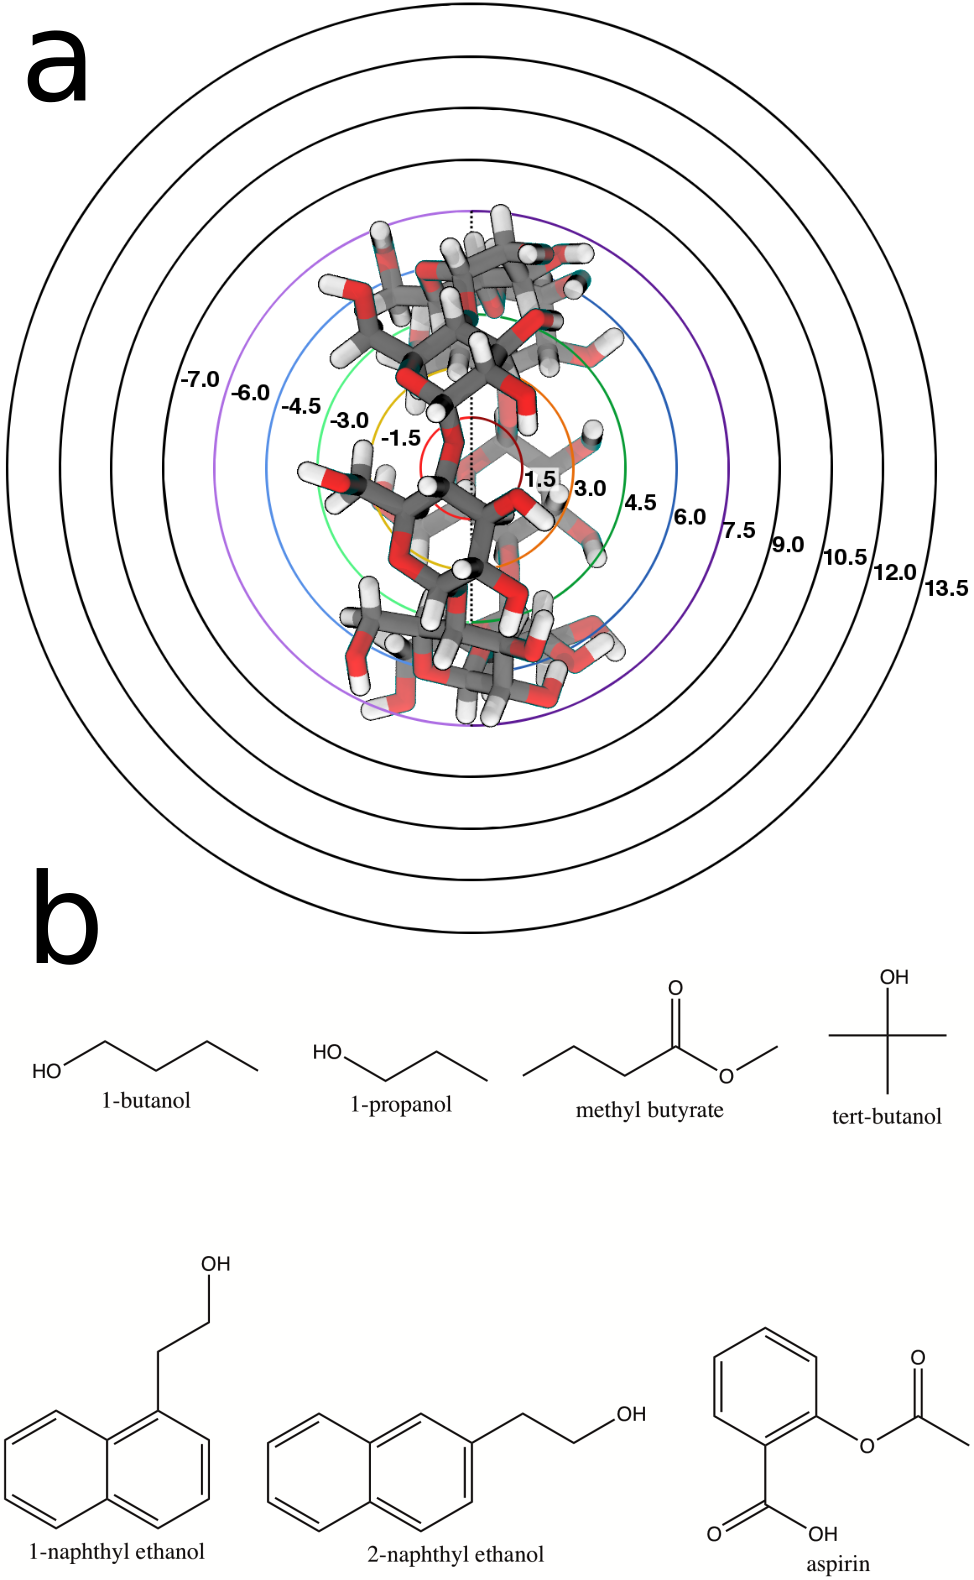
\includegraphics{images/bcdmilestones_comb_resize2.png}

	\caption{a) $\beta$-cyclodextrin with milestones spaced at 1.5~\AA increments and b) the seven ligands used in this study. The top four ligands are known to bind more weakly while the bottom three are known to bind more tightly.}
	\label{fig:BCD_ligands}
\end{figure} 


